\documentclass[a4paper, 12pt]{article}

% packages
\usepackage{amssymb}
\usepackage[fleqn]{mathtools}
\usepackage{tikz}
\usepackage{enumerate}
\usepackage{bussproofs}
\usepackage{xcolor}
\usepackage[margin=1.3cm]{geometry}
\usepackage{logicproof}
\usepackage{diagbox}
\usepackage{listings}
\usepackage{graphicx}
\usepackage{lstautogobble}
\usepackage{hyperref}
\usepackage{multirow}
\usepackage{tipa}
\usepackage{pgfplots}
\usepackage{adjustbox}

% tikz libraries
\usetikzlibrary{
    decorations.pathreplacing,
    arrows,
    shapes,
    shapes.gates.logic.US,
    circuits.logic.US,
    calc,
    automata,
    positioning,
    intersections
}

\pgfplotsset{compat=1.16}

\pgfmathdeclarefunction{gauss}{2}{%
  \pgfmathparse{1/(#2*sqrt(2*pi))*exp(-((x-#1)^2)/(2*#2^2))}%
}

\allowdisplaybreaks % allow environments to break
\setlength\parindent{0pt} % no indent

% shorthand for verbatim
% this clashes with logicproof, so maybe fix this at some point?
\catcode`~=\active
\def~#1~{\texttt{#1}}

% code listing
\lstdefinestyle{main}{
    numberstyle=\tiny,
    breaklines=true,
    showspaces=false,
    showstringspaces=false,
    tabsize=2,
    numbers=left,
    basicstyle=\ttfamily,
    columns=fixed,
    fontadjust=true,
    basewidth=0.5em,
    autogobble,
    xleftmargin=3.0ex,
    mathescape=true
}
\newcommand{\dollar}{\mbox{\textdollar}} %
\lstset{style=main}

% augmented matrix
\makeatletter
\renewcommand*\env@matrix[1][*\c@MaxMatrixCols c]{%
\hskip -\arraycolsep
\let\@ifnextchar\new@ifnextchar
\array{#1}}
\makeatother

% ceiling / floor
\DeclarePairedDelimiter{\ceil}{\lceil}{\rceil}
\DeclarePairedDelimiter{\floor}{\lfloor}{\rfloor}

% custom commands
\newcommand{\indefint}[2]{\int #1 \, \mathrm{d}#2}
\newcommand{\defint}[4]{\int_{#1}^{#2} #3 \, \mathrm{d}#4}
\newcommand{\pdif}[2]{\frac{\partial #1}{\partial #2}}
\newcommand{\dif}[2]{\frac{\mathrm{d}#1}{\mathrm{d}#2}}
\newcommand{\limit}[2]{\raisebox{0.5ex}{\scalebox{0.8}{$\displaystyle{\lim_{#1 \to #2}}$}}}
\newcommand{\limitsup}[2]{\raisebox{0.5ex}{\scalebox{0.8}{$\displaystyle{\limsup_{#1 \to #2}}$}}}
\newcommand{\summation}[2]{\sum\limits_{#1}^{#2}}
\newcommand{\product}[2]{\prod\limits_{#1}^{#2}}
\newcommand{\intbracket}[3]{\left[#3\right]_{#1}^{#2}}
\newcommand{\laplace}{\mathcal{L}}
\newcommand{\fourier}{\mathcal{F}}
\newcommand{\mat}[1]{\boldsymbol{#1}}
\renewcommand{\vec}[1]{\boldsymbol{#1}}
\newcommand{\rowt}[1]{\begin{bmatrix}
    #1
\end{bmatrix}^\top}
\DeclareMathOperator*{\argmax}{argmax}
\DeclareMathOperator*{\argmin}{argmin}

\newcommand{\lto}[0]{\leadsto\ }

\newcommand{\ulsmash}[1]{\underline{\smash{#1}}}

\newcommand{\powerset}[0]{\wp}
\renewcommand{\emptyset}[0]{\varnothing}

\makeatletter
\newsavebox{\@brx}
\newcommand{\llangle}[1][]{\savebox{\@brx}{\(\m@th{#1\langle}\)}%
  \mathopen{\copy\@brx\kern-0.5\wd\@brx\usebox{\@brx}}}
\newcommand{\rrangle}[1][]{\savebox{\@brx}{\(\m@th{#1\rangle}\)}%
  \mathclose{\copy\@brx\kern-0.5\wd\@brx\usebox{\@brx}}}
\makeatother
\newcommand{\lla}{\llangle}
\newcommand{\rra}{\rrangle}
\newcommand{\la}{\langle}
\newcommand{\ra}{\rangle}
\newcommand{\crnr}[1]{\text{\textopencorner} #1 \text{\textcorner}}
\newcommand{\bnfsep}[0]{\ |\ }
\newcommand{\concsep}[0]{\ ||\ }

\newcommand{\axiom}[1]{\AxiomC{#1}}
\newcommand{\unary}[1]{\UnaryInfC{#1}}
\newcommand{\binary}[1]{\BinaryInfC{#1}}
\newcommand{\trinary}[1]{\TrinaryInfC{#1}}
\newcommand{\quaternary}[1]{\QuaternaryInfC{#1}}
\newcommand{\quinary}[1]{\QuinaryInfC{#1}}
\newcommand{\dproof}[0]{\DisplayProof}
\newcommand{\llabel}[1]{\LeftLabel{\scriptsize #1}}
\newcommand{\rlabel}[1]{\RightLabel{\scriptsize #1}}

\newcommand{\ttbs}{\char`\\}
\newcommand{\lrbt}[0]{\ \bullet\ }

% colours
\newcommand{\violet}[1]{\textcolor{violet}{#1}}
\newcommand{\blue}[1]{\textcolor{blue}{#1}}
\newcommand{\red}[1]{\textcolor{red}{#1}}
\newcommand{\teal}[1]{\textcolor{teal}{#1}}

% reasoning proofs
\usepackage{ltablex}
\usepackage{environ}
\keepXColumns
\NewEnviron{reasoning}{
    \begin{tabularx}{\textwidth}{rlX}
        \BODY
    \end{tabularx}
}
\newcommand{\proofline}[3]{$(#1)$ & $#2$ & \hfill #3 \smallskip \\}
\newcommand{\proofarbitrary}[1]{& take arbitrary $#1$ \smallskip \\}
\newcommand{\prooftext}[1]{\multicolumn{3}{l}{#1} \smallskip \\}
\newcommand{\proofmath}[3]{$#1$ & = $#2$ & \hfill #3 \smallskip \\}
\newcommand{\prooftherefore}[1]{& $\therefore #1$ \smallskip \\}
\newcommand{\proofbc}[0]{\prooftext{\textbf{Base Case}}}
\newcommand{\proofis}[0]{\prooftext{\textbf{Inductive Step}}}

% ER diagrams
\newcommand{\nattribute}[4]{
    \node[draw, state, inner sep=0cm, minimum size=0.2cm, label=#3:{#4}] (#1) at (#2) {};
}
\newcommand{\mattribute}[4]{
    \node[draw, state, accepting, inner sep=0cm, minimum size=0.2cm, label=#3:{#4}] (#1) at (#2) {};
}
\newcommand{\dattribute}[4]{
    \node[draw, state, dashed, inner sep=0cm, minimum size=0.2cm, label=#3:{#4}] (#1) at (#2) {};
}
\newcommand{\entity}[3]{
    \node[] (#1-c) at (#2) {#3};
    \node[inner sep=0cm] (#1-l) at ($(#1-c) + (-1, 0)$) {};
    \node[inner sep=0cm] (#1-r) at ($(#1-c) + (1, 0)$) {};
    \node[inner sep=0cm] (#1-u) at ($(#1-c) + (0, 0.5)$) {};
    \node[inner sep=0cm] (#1-d) at ($(#1-c) + (0, -0.5)$) {};
    \draw
    ($(#1-c) + (-1, 0.5)$) -- ($(#1-c) + (1, 0.5)$) -- ($(#1-c) + (1, -0.5)$) -- ($(#1-c) + (-1, -0.5)$) -- cycle;
}
\newcommand{\relationship}[3]{
    \node[] (#1-c) at (#2) {#3};
    \node[inner sep=0cm] (#1-l) at ($(#1-c) + (-1, 0)$) {};
    \node[inner sep=0cm] (#1-r) at ($(#1-c) + (1, 0)$) {};
    \node[inner sep=0cm] (#1-u) at ($(#1-c) + (0, 1)$) {};
    \node[inner sep=0cm] (#1-d) at ($(#1-c) + (0, -1)$) {};
    \draw
    ($(#1-c) + (-1, 0)$) -- ($(#1-c) + (0, 1)$) -- ($(#1-c) + (1, 0)$) -- ($(#1-c) + (0, -1)$) -- cycle;
}

% AVL Trees
\newcommand{\avltri}[4]{
    \draw ($(#1)$) -- ($(#1) + #4*(0.5, -1)$) -- ($(#1) + #4*(-0.5, -1)$) -- cycle;
    \node at ($(#1) + #4*(0, -1) + (0, 0.5)$) {#3};
    \node at ($(#1) + #4*(0, -1) + (0, -0.5)$) {#2};
}

% RB Trees
\tikzset{rbtr/.style={inner sep=2pt, circle, draw=black, fill=red}}
\tikzset{rbtb/.style={inner sep=2pt, circle, draw=black, fill=black}}

% Samples
\tikzset{spos/.style={inner sep=2pt, circle, draw=black, fill=blue!20}}
\tikzset{sneg/.style={inner sep=2pt, circle, draw=black, fill=red!20}}

% actual document
\begin{document}
    {\sc Computing $3^\text{rd}$ Year Notes} \hfill ~https://github.com/lin-e/imperial-revision~
    \rule{\textwidth}{0.1pt}
    \section*{CO343 - Operations Research \hfill (60016)}
        \subsection*{Lecture 1}
            Operations research is the science of taking decisions, it's a branch of applied mathematics where we attempt to model problems where need to make a decision.
            The decisions aren't arbitrary, and we want to attempt to score each decision based on some metric (such as time, cost, etc.), to find the optimal solution.
            \medskip

            The course focuses on formulating a mathematical model to represent the problem, and then developing a computer-based procedure for deriving solutions to the problem from the model.
            Assume our goal was the following;
            $$\min_{\vec{x}} z = f(\vec{x}) \hspace{50pt} \text{subject to } \vec{x} \in \mathcal{X}$$
            \begin{itemize}
                \itemsep0em
                \item \textbf{decision variables} \hfill $\vec{x} \in \mathbb{R}^n$
                \item \textbf{objective function} \hfill $f : \mathbb{R}^n \to \mathbb{R}$
                \item \textbf{feasible set} (set of admissible decisions) \hfill $\mathcal{X} \subseteq \mathbb{R}^n$
                \item \textbf{optimal solution} (any vector that minimises $f$) \hfill $\vec{x^*}$
                \item \textbf{optimal value} \hfill $z^* = f(\vec{x^*})$
            \end{itemize}
            \subsubsection*{Linear Programming}
                A linear program optimises a \textbf{linear objective function}, where a feasible set is described by linear equality / inequality constraints.
                Compared to non-linear problems, where a \textbf{local} maximum may vary (and therefore be sub-optimal) depending on the starting search position, this isn't a concern for linear problems.
                \medskip

                We can say the polygon representing a two dimensional feasible set is convex if the points on the line joining two points in the feasible set are also in the polygon.
                If this region is convex and linear, it can be proven that a local optimum is also a global optimum.
                For example, take $x$ and $x^\prime$;
                \begin{center}
                    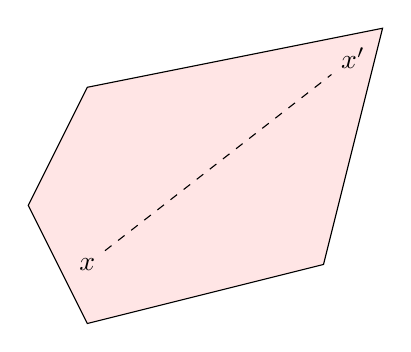
\begin{tikzpicture}[x=0.75cm, y=0.75cm]
                        \draw[fill=red!10]
                        (0, 0) -- (5, 1) -- (4, -3) -- (0, -4) -- (-1, -2) -- cycle;

                        \node (x) at (0, -3) {$x$};
                        \node (xp) at (4.5, 0.5) {$x^\prime$};

                        \draw (x) edge[dashed] (xp);
                    \end{tikzpicture}
                \end{center}
            \subsubsection*{Linear Programming Example}
                A manufacturer produces $A$ (acid) and $C$ (caustic) and wants to decide a production plan.
                The ingredients for $A$ and $C$ are $X$ (a sulphate) and $Y$ (sodium).
                \begin{itemize}
                    \itemsep0em
                    \item each ton of $A$ requires 2 tons of $X$ and 1 ton of $Y$
                    \item each ton of $C$ requires 1 ton of $X$ and 3 tons of $Y$
                    \item supply of $X$ is limited to 11 tons per week
                    \item supply of $Y$ is limited to 18 tons per week
                    \item $A$ sells for £1000 per ton
                    \item $C$ sells for £1000 per ton
                    \item a maximum of 4 tons of $A$ can be sold per week
                \end{itemize}
                Our goal is to maximise weekly value of sales of $A$ and $C$.
                To determine how much $A$ and $C$ to produce, we need to formulate a \textbf{mathematical programming model};
                \begin{itemize}
                    \itemsep0em
                    \item \textbf{decision variables}
                        \begin{itemize}
                            \itemsep0em
                            \item weekly production of $A$ (tons) \hfill $x_1$
                            \item weekly production of $B$ (tons) \hfill $x_2$
                        \end{itemize}
                    \item \textbf{objective function} (weekly profit in £1000s) \hfill $z = f(x_1, x_2)$
                    \item \textbf{feasible set} \hfill $\vec{x} = (x_1, x_2) \in \mathcal{X}$
                \end{itemize}
                A \textbf{production plan} is representable as $\vec{x} = (x_1, x_2)$.
                The objective function can be written as $z = x_1 + x_2$.
                Another constraint is that \violet{$x_1 \geq 0$} and \violet{$x_2 \geq 0$}; we cannot produce a negative amount of a product.
                $x_1$ tons of $A$ and $x_2$ tons of $C$ requires $2x_1 + x_2$ tons of $X$, and we know that is limited to 11 tons per week; therefore we have the constraint \blue{$2x_1 + x_2 \leq 11$}.
                Similarly, we also have the limitation of \red{$x_1 + 3x_2 \leq 18$}, because of the limitations of $Y$.
                Finally, we have another restriction that we cannot sell more than 4 tons of $A$, therefore \teal{$x_1 \leq 4$}.
                \medskip

                To get the overall feasible set, we intersect the feasible set of all the constraints to get the following;
                \begin{center}
                    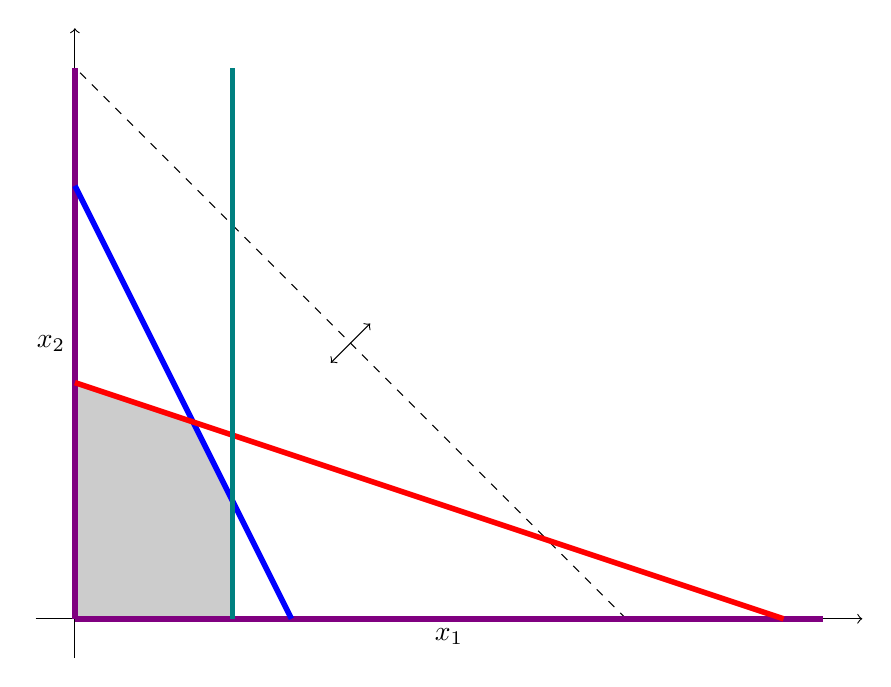
\begin{tikzpicture}[x=0.5cm, y=0.5cm]
                        \draw
                        (0, -1) edge[->, left] node{$x_2$} (0, 15)
                        (-1, 0) edge[->, below] node{$x_1$} (20, 0);

                        \draw
                        (14, 0) edge[dashed] (0, 14)
                        (6.5, 6.5) edge[<->] (7.5, 7.5);

                        \draw[fill=black!20] (0, 0) -- (0, 6) -- (3, 5) -- (4, 3) -- (4, 0) -- cycle;

                        \draw
                        (0, 0) edge[violet, line width=2pt] (0, 14)
                        (0, 0) edge[violet, line width=2pt] (19, 0)
                        (0, 11) edge[blue, line width=2pt] (5.5, 0)
                        (0, 6) edge[red, line width=2pt] (18, 0)
                        (4, 0) edge[teal, line width=2pt] (4, 14);
                    \end{tikzpicture}
                \end{center}
                Each of the following vertices is the intersection of constraints, which can be obtained by solving the linear equation of each line;
                \begin{align*}
                    O & = (0, 0) \\
                    P & = (0, 6) \\
                    Q & = (3, 5) \\
                    R & = (4, 3) \\
                    S & = (4, 0)
                \end{align*}
                By moving the objective function (the dashed line), in the direction of the arrows, we can see that the $z$ value increases further away from the origin, and therefore the graphical result that results in the highest value is $Q$.
                Typically the optimal solution lies on a vertex, however in some cases, there can be multiple solutions (an edge when the objective function is parallel to the constraint, or all the points in the feasible set in the case of a constant objective function).
                \medskip

                The simplest algorithm is to enumerate all the vertices (intersections) of the feasible set, however this can have exponential complexity in the worst case and the number of vertices grow quite quickly in higher dimensions.
                The \textbf{Simplex Algorithm} finds an optimal vertex, often inspecting a \textbf{small subset} of the total.
                \medskip

                We can vary this example, for example if we wanted to minimise $z = 3x_1 - x_2$ over the feasible set, we can examine the objective function at each of the vertices;
                \begin{center}
                    \begin{tabular}{c|c|c|c|c}
                        $O = (0, 0)$ & $P = (0, 6)$ & $Q = (3, 5)$ & $R = (4, 3)$ & $S = (4, 0)$ \\
                        \hline
                        0 & -6 & 4 & 9 & 12
                    \end{tabular}
                \end{center}
                This therefore gives us $P = (x_1, x_2) = (0, 6)$ as the optimal.
                \medskip

                On the other hand, if we were to maximise $z = 2x_1 + x_2$, any point on the line segment $QR$ would be optimal; this tells us that points other than the vertices can be optimal, but there is at least one optimal vertex.
                \medskip

                Additionally, if we were to set a production goal of 7 tons of $A$, we'd have an empty feasible set, since $x_1 \geq 7$ would cause an empty set with $x_1 \leq 4$.
                In this case, the LP is \textbf{infeasible}.
                Similarly, if the constraints on $X$ and $Y$ were removed, the objective function could grow to $+\infty$, hence the LP is \textbf{unbounded}.
        \subsection*{Lecture 2}
            \subsubsection*{Standard Form}
                In order to use a computer to solve an LP problem, we need to define a \textbf{standard form};
                \begin{itemize}
                    \itemsep0em
                    \item the goal is to \textbf{minimise} a \textbf{linear} objective function
                    \item all constraints are linear equality constraints
                    \item all constraint right hand sides are non-negative
                    \item all decision variables are non-negative
                \end{itemize}
                A linear problem in standard form is as follows;
                $$\begin{matrix}
                    \text{minimise} & z = c_1 x_1 & + & c_2 x_2 & + & \cdots & c_n x_n \\ \\
                    \text{subject to} & a_{1, 1} x_1 & + & a_{1, 2} x_2 & + & \cdots & a_{1, n} x_n & = & b_1 \\
                    & a_{2, 1} x_1 & + & a_{2, 2} x_2 & + & \cdots & a_{2, n} x_n & = & b_2 \\
                    & \vdots & & \vdots & & & \vdots & & \vdots \\
                    & a_{m, 1} x_1 & + & a_{m, 2} x_2 & + & \cdots & a_{m, n} x_n & = & b_m
                \end{matrix}$$
                This has the constraints that all decision variables $\forall i \in [1, n]\ x_i \geq 0$ and $\forall i \in [1, m]\ b_i \geq 0$.
                The \textbf{input parameters} $b_i$, $c_j$, and $a_{i, j}$ are fixed real constants.
                Clearly, this can be written more compactly as the following;
                \begin{align*}
                    \mat{A} & = \begin{bmatrix}
                        a_{1, 1} & a_{1, 2} & \cdots & a_{1, n} \\
                        a_{2, 1} & a_{2, 2} & \cdots & a_{2, n} \\
                        \vdots & \vdots & \ddots & \vdots \\
                        a_{m ,1} & a_{m, 2} & \cdots & a_{m, n}
                    \end{bmatrix} \\
                    \vec{b} & = \begin{bmatrix}
                        b_1 \\ b_2 \\ \vdots \\ b_m
                    \end{bmatrix} \\
                    \vec{x} & = \begin{bmatrix}
                        x_1 \\ x_2 \\ \vdots \\ x_n
                    \end{bmatrix} \\
                    \vec{c} & = \begin{bmatrix}
                        c_1 \\ c_2 \\ \vdots \\ c_n
                    \end{bmatrix}
                \end{align*}
                Therefore, the equation can be written as;
                $$\text{minimise } \vec{z} = \vec{c}^\top \vec{x} \text{ subject to } \mat{A}\vec{x} = \vec{b}$$
                Note that $\vec{x} \geq 0$ and $\vec{b} \geq 0$, which means that it holds \textbf{component-wise} (such that $\forall x_i \in \vec{x}\ x_i \geq 0$).
            \subsubsection*{Standardising}
                This follows the example in tutorial 1.
                \medskip

                Our goal is to maximise $y = 2x_1 + x_2$, (s.t.) subject to;
                \begin{itemize}
                    \itemsep0em
                    \item $x_1 - 4x_2 \leq 1$
                    \item $-x_1 - 5x_2 \leq -3$
                    \item $x_1, x_2 \geq 0$
                \end{itemize}
                We can do the following conversion steps to get the equations into the standard form.
                To reformulate inequalities as equalities, we introduced the \textbf{slack variables} $s_1$ and $s_2$.
                All that is left to do is to convert the maximisation into a minimisation, which can be done by negating the objective function.
                \begin{align*}
                    x_1 - 4x_2 & \leq 1 & \Rightarrow \\
                    x_1 - 4x_2 + \violet{s_1} & = 1 \\
                    -x_1 - 5x_2 & \leq 3 & \Rightarrow \\
                    x_1 + 5x_2 & \geq -3 & \Rightarrow \\
                    x_1 + 5x_2 - \blue{s_2} & = -3 \\
                    x_1, x_2, \violet{s_1}, \blue{s_2} & \geq 0 \\
                    \text{(maximise) } y & = 2x_1 + x_2 & \Rightarrow \\
                    \text{(minimise) } z & = -2x_1 - x_2
                \end{align*}
                Therefore, we can therefore say a minimisation of $\vec{z} = \vec{c}^\top\vec{x}$ subject to $\mat{A}\vec{x} \leq \vec{b}$ and $\vec{x} \geq 0$ is equivalent to the same minimisation subject to $\mat{A}\vec{x} + \vec{s} = \vec{b}$ and $\vec{x}, \vec{s} \geq 0$.
                The slack variables take the value of the difference $\vec{b} - \mat{A}\vec{x}$.
                Similarly, \textbf{excess variables} are the same, but instead of being added to the left hand side of the inequality, they are subtracted, and therefore take the value of the difference $\mat{A}\vec{x} - \vec{b}$.
                Additionally, a change of sign for the right hand side is trivial, as it can be done by multiplying the entire inequality by $-1$.
            \subsubsection*{Free Variables}
                Suppose the constraint $x_j \geq 0$ does not exist, such that it can be positive or negative.
                We can do this by substituting $x_j = x_j^+ - x_j^-$.
                The LP now has the following $n + 1$ variables;
                $$x_1, \dots, x_{j - 1}, x_j^+, x_j^-, x_{j + 1}, \dots, x_n$$
                Another approach to introduce free variables is to use substitution.
                Any \textbf{equality constraint} involving $x_j$ can be used to eliminate $x_j$, as for $x_1$ in the following conditions (with the substitution of $x_1 = 5 - 3x_2 - x_3$);
                \begin{align*}
                    \text{(minimise) } z & = x_1 + 3x_2 + 4x_3 \\
                    x_1 + 2x_2 + x_3 & = 5 \\
                    2x_1 + 3x_2 + x_3 & = 6 & \Rightarrow \\ \\
                    \violet{\text{(minimise) } z} &\ \violet{= x_2 + 3x_3 + 5} \\
                    \violet{x_2 + x_3} &\ \violet{= 4}
                \end{align*}
            \subsubsection*{Tutorial}
                \begin{enumerate}[1.]
                    \itemsep0em
                    \setcounter{enumi}{1}
                    \item
                        A company produces laptops at two factories, $A$ and $B$.
                        In factory $A$, $s_A$ laptops are produced a year, and $s_B$ laptops are produced a year in factory $B$.
                        The three stores, 1, 2, and 3, sell $d_1$, $d_2$, and $d_3$ a year.
                        The cost of shipping a laptop from the factory $i \in \{A, B\}$ to store $j \in \{1, 2, 3,\}$ is $c_{i, j}$.
                        Assume that the demand of all stores can be satisfied, such that $s_A + s_B \geq d_1 + d_2 + d_3$.
                        \begin{enumerate}[1.]
                            \itemsep0em
                            \item How should the laptops be shipped from the two factories to minimise shipping costs, assuming the following;
                                \begin{align*}
                                    \begin{bmatrix}
                                        s_A \\ s_B
                                    \end{bmatrix} & = \begin{bmatrix}
                                        3 \\ 3
                                    \end{bmatrix} \\
                                    \begin{bmatrix}
                                        d_1 \\ d_2 \\ d_3
                                    \end{bmatrix} & = \begin{bmatrix}
                                        2 \\ 2 \\ 2
                                    \end{bmatrix} \\
                                    (c_{i, j}) & = \begin{bmatrix}
                                        1 & 2 & 1 \\
                                        2 & 1 & 2
                                    \end{bmatrix} & \text{(first row corresponds to store $A$)}
                                \end{align*}
                            \item Formulate the optimisation model corresponding to the previous question, using the general parameters;
                                \medskip

                                Note that we will denote the number of laptops from each factory $i \in \{A, B\}$ to store $j \in \{1, 2, 3\}$ as $x_{i, j}$.
                                We therefore want to minimise the following;
                                $$z = \summation{i}{} \summation{j}{} c_{i, j}x_{i, j}$$
                                Under the following conditions;
                                \begin{align*}
                                    x_{A, j} + x_{B, j} & = d_j & \forall j \in \{1, 2, 3\} \\
                                    x_{i, 1} + x_{i, 2} + x_{i, 3} & \leq s_i & \forall i \in \{A, B\} \\
                                    x_{i, j} & \geq 0 & \forall i, \forall j
                                \end{align*}
                                It's important to note that satisfying demand is to use equality, as we can reduce the amount of computation we need to do.
                        \end{enumerate}
                \end{enumerate}
\end{document}